\section{Hydraulic circuits}
\label{sec:hydraulicCircuits}

\subsection{Head}

It was indicated before that the total hydraulic energy from equation
\ref{eq:hydraulicEnergy} is defined up to a constant. We can indeed
arbitrarily choose a reference position $z_0$ and pressure $p_0$
freely; typically $p_0$ is chosen to be the atmospheric pressure,
whereas a convenient reference position $z_0$ is chosen in function of
the installation, for instance the inlet of a pump.

The total hydraulic energy of the flow is in practice quantified per
unit of \emph{weight} rather than \emph{mass} through the \emph{total
  dynamic head} or \emph{height} \head, defined as
\begin{equation}
  \head = \frac{\eHydr}{\grav} = 
  \underbrace{\frac{\pres - \pres_0}{\dens g} + z - z_0}_{\head_m} + 
  \underbrace{\frac{\vel^2}{2 \grav}}_{\head_d}
  \label{eq:hydraulicHead}
\end{equation} 
The total dynamic head is further split into the \emph{static} or
\emph{manometric} head $\head_m$, combining pressure and elevation,
and the \emph{dynamic} or \emph{velocity head} $\head_d$,
corresponding to the kinetic energy.
\begin{figure}
  \centering{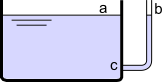
\includegraphics[width=0.3\textwidth]{hydrodynamics/manometer.png}}
  \caption{Manometric head measurement}
  \label{fig:head}
\end{figure}
The manometric head corresponds to the liquid column height $\head_m$
above a reference location $z_0$ at the reference pressure $p_0$, as
illustrated in figure \ref{fig:head}. Due to hydrostatic equilibrium,
we have
\begin{align*}
  \frac{p_a - p_0}{\dens \grav} + z_a - z_0 = \frac{p_b - p_0}{\dens \grav} + z_b - z_0 = \frac{p_c - p_0}{\dens \grav} + z_c - z_0 
\end{align*}
\todo{rework}
Setting $p_0$ to the atmospheric pressure and $z_0 = z_b$, we find
that the height of the water column with respect to the measurement
location $b$ corresponds to the pressure difference:
\begin{align*}
  \frac{p_c - p_b}{\dens \grav} = z_b - z_c
\end{align*}

\subsection{Major head losses}
\label{sec:hydraulicLosses}

The hydraulic losses in the circuit result from several phenomena, and
are typically computed using non-dimenional loss coefficients and the
bulk velocity
\begin{align*} 
  \vel_b &= \frac{4 \vFlow}{\pi D^2}
\end{align*}
The major losses are caused by wall friction in the pipes. 

For circular pipes with diameter $D$, the friction loss is computed
using the Darcy-Weisbach friction coefficient $\lambda$
\begin{equation}
  \loss_f = \lambda \frac{L}{D}~\frac{\vel_b^2}{2\grav}
  \label{eq:frictionLossDarcyWeisbach}
\end{equation}
which is a function of the pipe Reynolds number $Re_D = \vel_b D /
\kinVisc$. For the laminar regime, $\lambda$ follows from the
analytical solution for Poiseuille flow:
\begin{align}
  \lambda = \frac{64}{Re_D} 
  \label{eq:frictionFactorLaminar}
\end{align}
For the turbulent regime, the friction coefficient furthermore depends
on the roughness $\epsilon$ of the pipe, \eg through the implicit
correlation of Colebrook and White:
\begin{equation}
  \frac{1}{\sqrt{\lambda}} = -
  2~\log_{10}\left(\frac{\epsilon/D}{3.7} + \frac{2.51}{Re_D
      \sqrt{\lambda}}\right)
  \label{eq:frictionFactorColebrook}
\end{equation}
The transition from laminar to turbulent depends on the roughness. The
friction coefficient is summarized in the well-known Moody chart,
shown in figure \ref{fig:moody}. Notice that in the fully turbulent
regime, $\lambda$ becomes independent of the Reynolds number.
\begin{figure}[!h]
    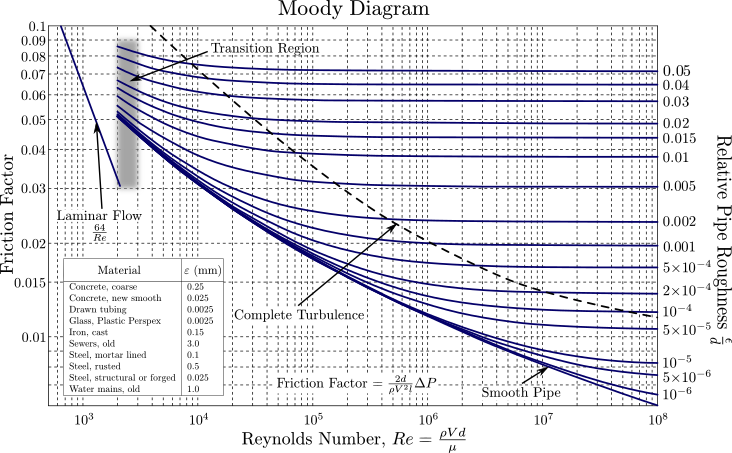
\includegraphics[width=\textwidth]{hydrodynamics/MoodyDiagram.png}
    \caption{Moody diagram - friction factor for pipe flow}
    \label{fig:moody}
  \caption{Determining hydraulic losses in a circuit. (Images from
    Wikimedia Commons)}
  \label{fig:hydraulicLosses}
\end{figure}
One difficulty related to the Colebrook-White equation is that it is
implicit. Therefore, quite a number of simpler correlations have been
proposed over the years (see \cite{wikipedia_darcy} for an
overview). For instance, the correlation proposed by Haaland is
\begin{equation}
  \frac{1}{\sqrt{\lambda}} = - 1.8
  \log_{10}\left(\left(\frac{\epsilon/D}{3.7}\right)^{1.11} +
    \frac{6.9}{Re_D}\right)
    \label{eq:haaland}
\end{equation}
providing an explicit, yet still complex, expression for $\lambda$.
Equations \ref{eq:frictionLossDarcyWeisbach} through
\ref{eq:haaland} are generalised to other pipe-like
configurations by replacing the diameter with the \emph{equivalent
  hydraulic diameter}
\begin{equation}
  D_h = \frac{4 S_h}{P_h}
\end{equation}
with $S_h$ the through-flow surface and $P_h$ its perimeter.
 
\subsection{Minor losses}

\begin{figure}[!h]
  \begin{subfigure}{0.65\textwidth}
    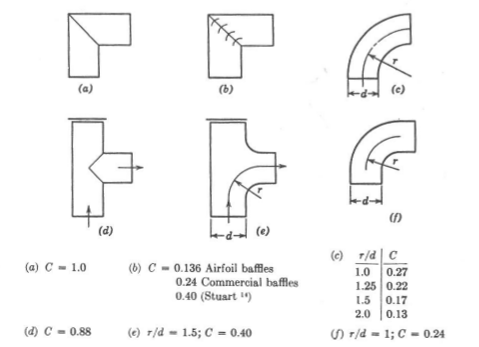
\includegraphics[width=\textwidth]{elbowLosses.png}
    \caption{Elbow losses, Stepanoff \cite{Stepanoff}}
  \end{subfigure}
  \begin{subfigure}{0.35\textwidth}
    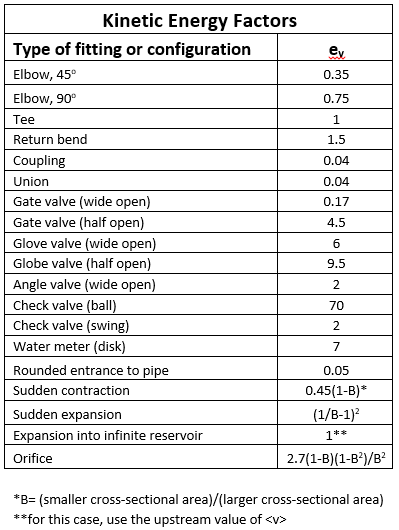
\includegraphics[width=\textwidth]{hydrodynamics/KineticEnergyFactors.png}
    \caption{Wikimedia}
  \end{subfigure}
  \caption{Kinetic energy factors}
  \label{fig:kineticEnergyFactors}
\end{figure}
The \emph{minor} or \emph{local losses} are associated to separation
and secondary flow losses in bends, expansions or restrictions,
junctions \ldots They are computed by formula of the form
\begin{equation}
  \loss = k_L \frac{\vel_b^2}{2\grav}
\end{equation}
With good approximation, the \emph{kinetic energy factors} $k_L$ can
be supposed independent of the Reynolds number and therefore listed in
a compendium, such as shown in figure
\ref{fig:kineticEnergyFactors}. Remark that the fluid loses all its
kinetic energy when discharging in a reservoir at rest, as indicated
by the corresponding kinetic energy factor $k_L=1$.

% A first example is the sudden expansion or otherwise known as the dump
% diffusion. Assuming the pipe section changes from the surface $A_1$ to
% $A_2$, we have the mass balance between station 1 and 2
% \begin{align*}
%     \vel_1 A_1 = \vel_2 A_2
% \end{align*}
% The momentum balance states that 
% \begin{align*}
%   (\pres_1 + \rho \vel_1^2) A_1 + \frac{\pres_1 + \rho
%     \pres_2}\left(A_2 - A_1\right) = \left(p_2 + \vel_2^2\right) A_2
% \end{align*}
% Combined, this gives us the total pressure loss
% \begin{align*}
%     p_{t2} - p_{t1} = \pres_2 + \dens \frac{\vel_2^2}{2} - \pres_1 + \dens \frac{\vel_1^2}{2}
% \end{align*}

% A second example concerns the losses generated by secondary flows in a
% pipe bend.

\subsection{Head diagram}

\begin{figure}
  \begin{subfigure}{\textwidth}
    \centering{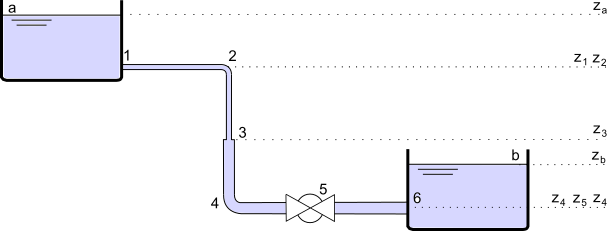
\includegraphics[width=0.85\textwidth]{hydrodynamics/hydraulicCircuit.png}}
    \caption{Circuit}
  \end{subfigure}
  \begin{subfigure}{\textwidth}
    \centering{
\tikzsetnextfilename{hydraulicCircuit}
\begin{tikzpicture}

  \scriptsize
  
  %% kinetic energy upstream & downstream
  \def\vU{12}
  \def\vD{4}
  \def\hA{400}

  %% dimensions

  \def\lPipeSB{15}
  \def\lPipeBE{10}
  \def\lPipeEB{10}
  \def\lPipeBV{10}
  \def\lPipeVD{15}
  
  \def\posReservoirA{5}
  \def\posIntake{\posReservoirA+10}
  \def\posBendU{\posIntake + \lPipeSB}
  \def\posExp{\posBendU + \lPipeBE}
  \def\posBendD{\posExp + \lPipeEB}
  \def\posValve{\posBendD + \lPipeBV}
  \def\posDischarge{\posValve + \lPipeVD}
  \def\posReservoirB{\posDischarge + 10}
  
  %% major losses
  
  \def\kPipe{0.2}
  \def\lossPipeSB{\kPipe*\lPipeSB*\vU}
  \def\lossPipeBE{\kPipe*\lPipeBE*\vU}
  \def\lossPipeEB{\kPipe*\lPipeEB*\vD}
  \def\lossPipeBV{\kPipe*\lPipeBV*\vD}
  \def\lossPipeVD{\kPipe*\lPipeVD*\vD}
  
  %% minor losses
  
  \def\kBend{0.75}
  \def\kSump{0.025}
  \def\kValve{6}
  \def\kDischarge{1}
  \def\kExp{1}
  
  \def\lossSump{\kSump*\vU}
  \def\lossBendU{\kBend*\vU}
  \def\lossExp{\kExp*\vU}
  \def\lossBendD{\kBend*\vD}
  \def\lossValve{\kValve*\vD}
  \def\lossDischarge{\kDischarge*\vD}

  %% positions in the head diagram

  \def\hSumpP{\hA}
  \def\hSumpM{\hSumpP - \lossSump}
  
  \def\hBendUP{\hSumpM - \lossPipeSB}
  \def\hBendUM{\hBendUP - \lossBendU}
  
  \def\hExpP{\hBendUM - \lossPipeBE}
  \def\hExpM{\hExpP - \lossExp}
  
  \def\hBendDP{\hExpM - \lossPipeEB}
  \def\hBendDM{\hBendDP - \lossBendD}
  
  \def\hValveP{\hBendDM - \lossPipeBV}
  \def\hValveM{\hValveP - \lossValve}

  \def\hDischargeP{\hValveM - \lossPipeVD}
  \def\hB{\hDischargeP - \vD}

  \def\hOffset{\hA - \hB}
  
  \begin{axis}[
    width = \textwidth, 
    height =0.3\textheight, 
    xtick = data, 
    xticklabels = {
      a, 
      Intake, 
      Bend,
      Expansion, 
      Bend,
      Valve, 
      Discharge, 
      b}, 
    ytick = \empty,
    axis lines = center, 
    xmin = 0, xmax = \posReservoirB+5, 
    ymin = \hB+\hOffset, ymax = \hA+\hOffset+40,
    xlabel = station,
    ylabel = $\head$,
    legend style   = {draw=none,anchor=west,at={(0.05,0.5)}},
    legend entries = {total head,static head},
    mark size = 1pt
    ],
    \addplot [mark=o,mark options={solid},black,line width=1pt] coordinates {
      (\posReservoirA,\hOffset + 20 +\hA)
      (\posIntake,\hOffset + 20 +\hSumpP) 
      (\posIntake,\hOffset + 20 +\hSumpM)
      (\posBendU,\hOffset + 20 +\hBendUP) 
      (\posBendU,\hOffset + 20 +\hBendUM) 
      (\posExp,\hOffset + 20 +\hExpP) 
      (\posExp,\hOffset + 20 +\hExpM) 
      (\posBendD,\hOffset + 20 +\hBendDP) 
      (\posBendD,\hOffset + 20 +\hBendDM) 
      (\posValve,\hOffset + 20 +\hValveP) 
      (\posValve,\hOffset + 20 +\hValveM) 
      (\posDischarge,\hOffset + 20 +\hDischargeP) 
      (\posReservoirB,\hOffset + 20 +\hB) 
    };
    
    \addplot [mark=o,mark options={solid},dashed,line width=1pt] coordinates {
      (\posReservoirA,\hOffset + 20 +\hA)
      (\posIntake,\hOffset + 20 +\hSumpP-\vU) 
      (\posIntake,\hOffset + 20 +\hSumpM-\vU)
      (\posBendU,\hOffset + 20 +\hBendUP-\vU) 
      (\posBendU,\hOffset + 20 +\hBendUM-\vU) 
      (\posExp,\hOffset + 20 +\hExpP-\vU) 
      (\posExp,\hOffset + 20 +\hExpM-\vD) 
      (\posBendD,\hOffset + 20 +\hBendDP-\vD) 
      (\posBendD,\hOffset + 20 +\hBendDM-\vD) 
      (\posValve,\hOffset + 20 +\hValveP-\vD) 
      (\posValve,\hOffset + 20 +\hValveM-\vD) 
      (\posDischarge,\hOffset + 20 +\hDischargeP-\vD) 
      (\posReservoirB,\hOffset + 20 +\hB) 
    };
    
    \addplot [dashed] coordinates {(0,\hOffset + 20 +\hA) (\posReservoirB,\hOffset + 20 +\hA)};
    \addplot [dashed] coordinates {(0,\hOffset + 20 +\hB) (\posReservoirB,\hOffset + 20 +\hB)};
    
    
    \addplot [dashed] coordinates {(\posReservoirA,\hOffset+\hB) (\posReservoirA,\hOffset+20+\hA)};
    \addplot [dashed] coordinates {(\posReservoirB,\hOffset+\hB) (\posReservoirB,\hOffset+20+\hA)};
    \addplot [dashed] coordinates {(\posBendU,\hOffset+\hB) (\posBendU,\hOffset+20+\hA)};
    \addplot [dashed] coordinates {(\posBendD,\hOffset+\hB) (\posBendD,\hOffset+20+\hA)};
    \addplot [dashed] coordinates {(\posExp,\hOffset+\hB) (\posExp,\hOffset+20+\hA)};
    \addplot [dashed] coordinates {(\posValve,\hOffset+\hB) (\posValve,\hOffset+20+\hA)};
    \addplot [dashed] coordinates {(\posDischarge,\hOffset+\hB) (\posDischarge,\hOffset+20+\hA)};
    \addplot [dashed] coordinates {(\posIntake,\hOffset+\hB) (\posIntake,\hOffset+20+\hA)};
    
    

    %\addplot [dashed] coordinates {(1.5,0) (1.5,\hS)};
    %\addplot [dashed] coordinates {(2.5,0) (2.5,\hI)};
    %\addplot [dashed] coordinates {(3.5,0) (3.5,\hO)};
    %\addplot [dashed] coordinates {(4.5,0) (4.5,\hD)};
    %\addplot [dashed] coordinates {(5.5,0) (5.5,\hB)};
    
    %\addplot [dashed] coordinates {(0,\hA) (5.6,\hA)}
    %node [pos=0.05,left,above]{$\head_a$};
    %\addplot [dashed] coordinates {(0,\hB) (5.6,\hB)}
    %node [pos=0.05,left,above]{$\head_b$};
    
    %\addplot [dashed] coordinates {(2.4,\hI) (4,\hI)};
    %\addplot [dashed] coordinates {(3.4,\hO) (5.6,\hO)};
    %\addplot [<->,>=latex] 
    %coordinates {(3.9,\hI) (3.9,\hO)} 
    %node [midway,right] {$\head_p$};
    %\addplot [<->,>=latex] 
    %coordinates {(5.5,\hB) (5.5,\hO)} 
    %node [midway,left] {$\loss_{ob}$};
    %\addplot [<->,>=latex] 
    %coordinates {(2.5,\hA) (2.5,\hI)} 
    %node [midway,left] {$\loss_{ai}$};
    
  \end{axis}

\end{tikzpicture}}
    \caption{EGL and HGL}
  \end{subfigure}
  \caption{A simple hydraulic circuit between reservoirs a and b,
    consisting of an inlet (1) and discharge (6), two 90$^\circ$ bends
    (2,4), a sudden expansion (3) and a ball valve (5).}
  \label{fig:headDiagramCircuit}
\end{figure}

The evolution of the total, static and dynamic head in a hydraulic
piping system is typically shown as a function of piping distance,
corresponding to major losses, and the location of specific components
resulting in localised minor losses or sudden head rises in the case
of pumps. The variation of pipe diameter is then reflected in the
change of dynamic head through the distance between the \emph{energy
  grade line (EGL)}, corresponding to total head, and the
\emph{hydraulic grade line (HGL)}, corresponding to static head.Figure
\ref{fig:headDiagramCircuit} shows a simple example of an EGL and HGL.

%%% Local Variables: 
%%% mode: latex
%%% TeX-master: t
%%% End: 
